% Setup - do not change
\documentclass[11pt]{article}
\usepackage[top=0.9in, left=0.9in, bottom=0.9in, right=0.9in]{geometry} 
\usepackage{parskip}

\usepackage[english]{babel}
\usepackage[utf8]{inputenc}
\usepackage{amsmath,amsthm,amssymb,graphicx,pdfpages,lipsum,hyperref}
\usepackage[none]{hyphenat}
\usepackage{csquotes}
\usepackage{multirow} 

\setlength\parindent{0pt}
%%%%%%%%%%%%%%%%%%%%%%%%%%%%%%%%%%%%%%%%%%%%%%%%%%%%%%%%%%%%%%%%%%%
% add other packages here if required

%% Bibliography are specified in this file. You can also choose inline bib style if you want to. But make sure your citation style is consistent (and proper)
% For more details on citation: https://library.unimelb.edu.au/recite
\usepackage[sorting = none]{biblatex}
\addbibresource{references.bib}

%%%%%%%%%%%%%%%%%%%%%%%%%%%%%%%%%%%%%%%%%%%%%%%%%%%%%%%%%%%%%%%%%%% the '%' symbol denotes comments

% Begin document creation
% DELETE THE \lipsum PLACEHOLDERS WHEN YOU BEGIN
\title{\textbf{The Impact of Weather on Usage Patterns of Different Modes of Transportation in New York City} \\ Predict the hourly demand of taxi and Citi bike in different weather}
\author{
Muhan Chu \\
Student ID: 1346862 \\
\href{https://github.com/MAST30034-AppliedDataScience/project-1-individual-MuhanChu}{Github repo with commit}
}

\begin{document}
\maketitle
\section{Introduction}
As the most populous city in the United States\cite{census} New York has a very diverse range of transportation options. In addition to traditional Taxi such as Yellow and Green Taxi, the Citi Bike, which was officially launched in 2013, has become very popular. Citi Bike provides NYC citizens with a more convenient and environmentally friendly way of traveling, but the new way of traveling may affect the demand of the traditional taxi service industry. It's not just the new modes of travel, the weather can also have an impact on travel patterns.

The question of this study is: How do weather factors affect the demand for Yellow Taxi, Green Taxi, and Citi Bike usage in New York City? To better investigate this question we will use data analysis and the creation of predictive models. First we collected data on Yellow taxi, Green Taxi, citiBike and New York City (NYC) weather. And after cleaning the data, then we performed Exploratory Data Analysis , including statistics and visualization of hourly travel demand in different weather conditions. Next. We also chose two prediction models, Linear regression model and Random Forest Regression model, to quantify the impact of weather factors on transportation choices.

This report provides recommendations for urban transportation planners, as well as taxi operators and bicycle system managers. Based on data analysis and prediction, it assists them in optimizing transportation scheduling and management to better meet the mobility needs of citizens . As well as balancing the relationship between the traditional taxi industry and the emerging bike-sharing system.

\subsection{Data set Introduction}
There are 4 main datasets examined in this report, the Yellow Taxi data set, the Green Taxi data set, the Citi Bike data set, and the Weather data set. The timeline here is from February 2023 to December 2023. This time period covers all seasons and is relatively long enough to see if there is a seasonal trend. This time period is also very time-sensitive and largely avoids the impact of COVID-19 on traffic conditions.

The Yellow and Green Taxi data set comes from the NYC Taxi \& Limousine Commission \cite{tlc}, which includes detailed data on boarding and alighting times, distance traveled, and various prices. Yellow Taxi mainly serves the main city of NYC, while Green Taxi covers the outer areas of New York City. Choosing these two types of taxi allows for a more comprehensive of taxi demand in NYC.

The Citi Bike data set is from Citi Bike System Data-NYC\cite{citibike}. This data set includes the start and end time of each trip, the street that the trip belongs to, and the user's membership status. Although this data set has relatively few attributes, the primary need for this study was the number of trips demanded, so this data was sufficient for the purpose of the study.

The weather data set, from the Visual Crossing weather\cite{visualcrossing}, includes data on time of day, temperature, wind, rainfall, snowfall, visibility and UV intensity, as well as the source of the data. This data set provides a very comprehensive view of the different dimensions of weather information in NYC.

The next table\ref{tab:dataset_summary} counts the initial shapes of the different datasets:
\begin{table}[h!]
\centering
\begin{tabular}{|l|c|c|}
\hline
\textbf{Data set} & \textbf{Number of Instance} & \textbf{Number of Attribute} \\ \hline
Yellow Taxi Data set & 35,243,460 & 19 \\ \hline
Green Taxi Data set & 718,849 & 20 \\ \hline
Citi Bike Data set & 33,311,618 & 13 \\ \hline
Weather Data set & 8,760 & 24 \\ \hline
\end{tabular}
\caption{The shape of dataset.}
\label{tab:dataset_summary}
\end{table}
\section{Preprocessing}
Before analyzing, we need to preprocess the data to ensure the quality and usefulness of the data. Next, we will introduce how to clean the data.
\subsection{Data Wrangling}
\subsubsection{For Taxi dataset}

\begin{itemize}
    \item Merge the Yellow and Green Taxi datasets. First, convert `lpep\_pickup\_datetime' to `tpep\_pickup\_datetime' and `lpep\_dropoff\_datetime' to `tpep\_dropoff\_datetime' in the Green Taxi dataset. Then, delete the `ehail\_fee' and `trip\_type' attributes from the Green Taxi dataset, and `airport\_fee' from the Yellow Taxi dataset. Now, the attributes in both datasets are the same.
    \item Remove duplicated instances,avoid repeated statistics.
    \item Delete rows where the number of passengers is greater than 6 or less than 0, which represents the range of passengers allowed in a taxi.
    \item Delete rows where `payment\_type' is not a value between 1 and 6
    \item Delete rows where `trip\_distance' is less than 0, as we consider these trips to be invalid.
    \item Delete records where any monetary value is less than 0, as these are considered invalid.
    \item Filter out data that does not fall within the time range of February to December 2023.
    \item Create a new attribute `duration' by subtracting `tpep\_pickup\_datetime' from `tpep\_dropoff\_datetime' in the dataset.
    \item Delete rows where the ``duration'' is less than 0.
\end{itemize}
In this study the main study is the hourly taxi demand, so the price study is not the main purpose of this study, but here the data is deleted to ensure the readability of the data.The total data of  Yellow and Green Taxi dataset was originally 35862309 instance, 18 Attribute. after finishing the above data cleaning steps, the data totaled 33177826 instances, 19 Attribute. Totaling 7.75\% of the data was deleted.

\subsubsection{For Citi Bike dataset}
\begin{itemize}
    \item Filter the latitude and longitude data\cite{latlong}.The range of Latitude in NYC is from 40.4774 to 40.9176 and the range of Longitude is from -74.2591 to -73.7004 and delete the data which is not in NYC.
    \item Filter the values of Timeline that are not in the required range.
    \item Create new Attribute `duration', subtract `started\_at' from `ended\_at'.
    \item Filter instances with `duration' less than 0
\end{itemize}
After the above data cleanup, the number of Instance is down to 33286027 and the number of instances is 14. In total, 0.0768\% of the data was removed.

\subsubsection{NYC weather data}
\begin{itemize}
    \item Modify the missing data for `preciptype'. Convert `null' to `not rain ' to try to unify the data types
    \item Unify the format of `datetime'. Unify the time description to `yyyy-MM-dd HH:mm:ss' format.
    \item Filter `datetime' to ensure that the time range is within the requirement. When reading the data, the weather data is read for the whole year 2023, so it needs to be filtered.
\end{itemize}
After the above data cleansing, data set retains 8016 instances and 24 Attributes.

\subsection{Feature Engineering and Feature Selection}
\begin{itemize}
    \item Split taxi, citi bike, weather dataset into 9 months and 2 months. We focus on the patterns of the first 9 months of data.
    \item Add `hour' to the three main aggregates based on `tpep\_pickup\_datetime', `started\_at', `datetime' and `time'. Add `hour', `day\_of\_week', `date'.
    \item Add  the taxi and citi bike dataset to be counted according to `date' and `hour' respectively to generate `citybike\_count' and `taxi\_count' respectively.
    \item Only the `count’, `hour’, and `day\_of\_week' data are kept in the four datasets. Since our research question is mainly about the impact of weather on taxi demand and Citi bike demand, only these three Attributes are retained
    \item Join the weather data with the taxi dataset and CitiBike dateset based on `date' and `hour' respectively.
\end{itemize}
The next step will be to look at the correlation between the data and our goal `taxi\_count' and `cityBike\_count' based on the first nine months of data, as well as the correlation between the correlation. Base on this ,to do the Feature Selection:
\begin{itemize}
    \item For categorical data, I used the chi-square test to calculate their correlation with the count data, and removed the categorical attribute with a p-value less than 0.05, which means the correlation is not strong.
    \item For numerical data, we selected one of the values with high correlation between attributes for deletion. The attribute with high correlation with the goal is kept.
\end{itemize}
Next table\ref{tab:combined_data} is the number of instances and attributes for each data set after feature engineering and feature selection, and the names of the retained attributes:
\renewcommand{\arraystretch}{1.5}
\begin{table}[h!]
\centering
\begin{tabular}{|l|c|p{8cm}|}
\hline
\textbf{Name of data set} & \textbf{Shape} & \textbf{Attribute Name} \\ \hline
Combined\_taxi\_weather\_9 & 10*6551 & \multirow{2}{8cm}{'hour', 'temp', 'humidity', 'preciptype', 'windgust', 'visibility', 'solarenergy', 'icon', 'day\_of\_week', 'taxi\_count'} \\ \cline{1-2}
Combined\_taxi\_weather\_2 & 10*1489 & \\ \hline
Combined\_citiBike\_weather\_9 & 11*6551 & \multirow{2}{8cm}{'hour', 'temp', 'dew', 'humidity', 'windgust', 'cloudcover', 'visibility', 'solarenergy', 'uvindex', 'severerisk', 'citibike\_count'} \\ \cline{1-2}
Combined\_citiBike\_weather\_2 & 11*1489 & \\ \hline
\end{tabular}
\caption{Summary of the combined weather and transportation datasets.}
\label{tab:combined_data}
\end{table}


\section{Analysis and Geospatial Visualisation}
\subsection{Time trend analysis}
Here we analyze the change of demand for taxi and Citi Bike over time, which cover both seasonal and long term trends \ref{fig:1}. Analyzing the overall trend the demand for taxi is relatively more stable and there are cyclical variations. These changes are somewhat linked to weekends or weekdays. The demand for Citi Bikes, does not have a clear pattern of change and the demand is not very stable.

Next, some seasonal differences can be observed in the graph. In the winter from February to April, the demand for Taxi is much higher than the demand for citi Bike. This may be related to the colder weather in winter, where taxi would be a more comfortable option compared to citi Bike. Whereas in June through August which is the summer, the demand for citi bike is higher than Taxi. The weather becomes warmer and more suitable for riding conditions.

Some of the more extreme fluctuations can also be seen in the picture. In September, there were more ups and downs, and after checking the major events in September\cite{nycguide}, there were more major events,  which were held in New York City. This is something that is not considered in this report.
In conclusion, on this graph it is possible to see that there is some substitution between citiBike demand and taxi demand in certain seasons.

\begin{figure}[h!]
    \centering
    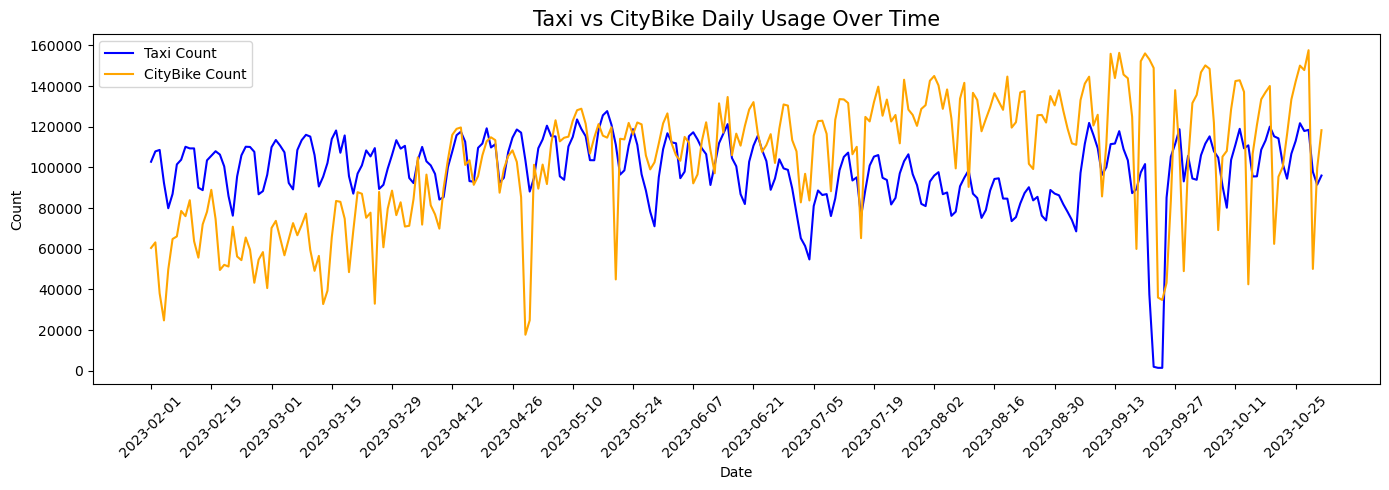
\includegraphics[width=1\textwidth]{plot/timeseries.png}
    \caption{Time trend of Taxi and Citi Bike demand}
    \label{fig:1}
\end{figure}

\subsection{Comparison of taxi and Citi Bike usage in weather conditions}
\begin{figure}[h!]
    \centering
    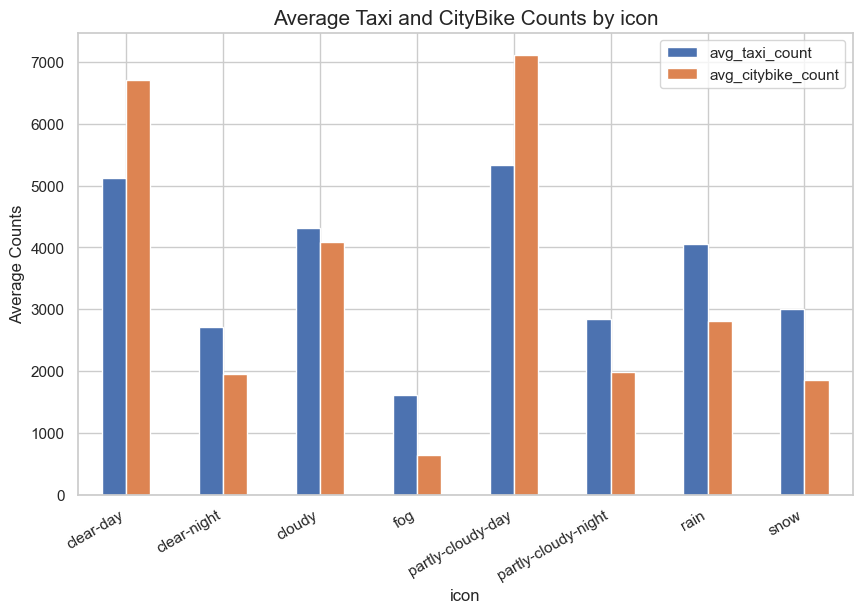
\includegraphics[width=0.5\textwidth]{plot/icon compare taxi and citi bike.png}
    \caption{Compare the average demand in different icon}
    \label{fig:2}
\end{figure}

Next, we analyze the demand for taxis versus Citi bikes under different weather conditions \ref{fig:2}. From the graph, it can be seen that except for cloudy days, there are some differences in all other types of weather. First of all, we can see that more people choose Citi Bike on both clear day and partly cloudy day. On the other hand, on clear night and partly cloudy night, more people choose taxis. This may be due to safety concerns, so more people choose to take a taxi. The data for foggy days also shows that bicycle usage is particularly low, probably because foggy days cause impaired visibility and make it less safe to ride.  But when the weather is relatively bad, more people choose to take a taxi, not only because the conditions for bicycling are not favorable, but also because safety is reduced.

Overall, it is not only the weather that has an impact on the choice of transportation mode of travel, but also the same daytime and nighttime. However, there is some unevenness in this report, as you can see from the next image that the number of times snow and fog occur is very low, and a small sample is not representative enough.

\subsection{Geographical Distribution Analysis }
The next step is to analyze the different NYC Taxi main boarding Taxi zones, from the picture\ref{fig:3}, the taxi boarding locations are mainly concentrated in the midtown and downtown Manhattan Island, and JFK Airport. Midtown and downtown Manhattan as the most prosperous places in New York, including Times Square and Fifth Avenue, Wall Street and the World Foreign Trade Center, resulting in these two areas of particularly high traffic, then these two areas also have the greatest demand for taxi. JFK Airport as the main transportation hub in New York, the flow of passengers is also very large.
\begin{figure}[h!]
    \centering
    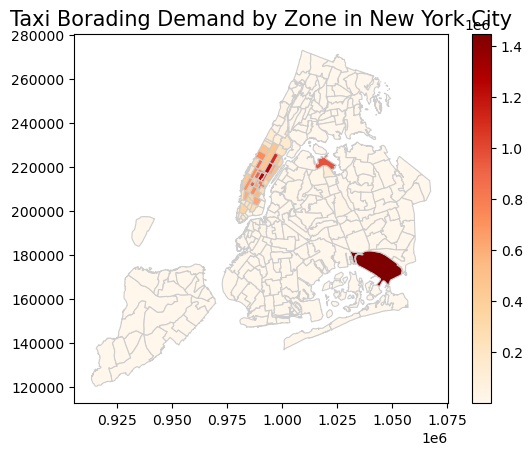
\includegraphics[width=0.5\textwidth]{plot/Taxi borading zone.png}
    \caption{Distribution of Taxi Boarding zone}
    \label{fig:3}
\end{figure}

Overall the areas of highest demand are similar for both taxi and Citi Bikes. They have high traffic volumes, high commercial activity, and are densely populated, making the demand for transportation in these areas very high. However, Citi Bike is often only used for short trips downtown, whereas Taxi's high-demand areas are not limited to downtown, but also include airport-related transportation hubs. 

\subsection{Distribution of Taxi Count and Citi Bike count}
This next graph\ref{fig:3} shows the distribution of Taxi\_count and Citi Bike count. the distribution of Citi Bike Count shows a right skew, with more demands being between 0-2000. This also suggests that demand for shared bikes is not stable, and there are cases where the longer right tail will produce very few cases where demand for bikes is particularly high. On the other hand, taxi demand distribution also showing a bit of a right skew, are mainly concentrated in the 4,000-8,000 range, suggesting that demand for taxi is a bit more stable. Based on such a distribution, here is a log\_transform of cityBike\_count and taxi\_count.
\begin{figure}[h!]
    \centering
    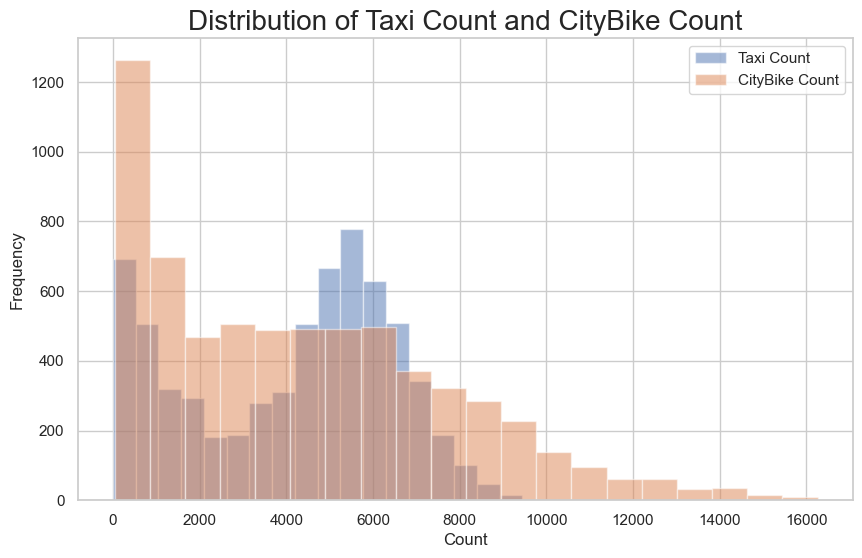
\includegraphics[width=0.5\textwidth]{plot/distribution of count.png}
    \caption{The distribution of taxi\_count and citi Bike count}
    \label{fig:4}
\end{figure}


\section{Modelling}
First of all, we divide the data into February to October 2023 as training data set and November to December 2023 as test data set. We use these factors that may affect the transportation demand to forecast the taxi and citi bike by demand in hourly. Here I have chosen two models Linear Regression and Random Forest regression, which require the data to be in the format of numerical data. I used one hot encoding to transform the categorical data, and performed the Min-max scale on all the numerical data to prevent individual feature ranges from having a large impact on the model.
\subsection{Linear regression model}
We model the prediction of taxi and Citi Bike demand based on the linear regression model of ordinary least squares \cite{LR}. Here we assume that all our Input attribute and output are linearly related, there is no correlation between the input Attribute, and the variance follows normal distribution. The previous feature selection and log transform are used to satisfy this condition. At the same time, cross validation was performed during model training, and the best model was selected to predict the test database. The models were evaluated using Root Square Error (RMSE) and R² values, RMSE was used to calculate the gap between the predicted and actual values of the model and R² values were used to calculate the goodness of fit of the model.
\subsection{Random forest regression model}
Random forest is an integrated learning method that makes predictions by constructing multiple decision trees and combining their outputs \cite{RFR}. Here I used 100 of random decision trees, using the maximum depth of the tree as hyper parameters, and modeling tuning for depths from 1-20 . Cross validation was also used to determine the best model. Finally a model that performs best on validation data set is used to predict the test data set. Here again RMSE and R-square are used to evaluate the models.

\section{Discussion}
\begin{table}[h!]
\centering
\begin{tabular}{|l|c|c|c|c|}
\hline
\multirow{2}{*}{} & \multicolumn{2}{c|}{\textbf{Linear Regression}} & \multicolumn{2}{c|}{\textbf{Random Forest Regression}} \\ \cline{2-5}
 & \textbf{RMSE} & \textbf{R-square} & \textbf{RMSE} & \textbf{R-square} \\ \hline
\textbf{Taxi count} & 0.4519 & 0.8037 & 0.3957 & 0.8395 \\ \hline
\textbf{Citi Bike count} & 0.4944 & 0.8188 & 0.5487 & 0.7768 \\ \hline
\end{tabular}
\caption{Comparison of Linear Regression and Random Forest Regression}
\label{tab:regression_comparison}
\end{table}
From this table used for comparison [table 4], it can be seen that the Random Forest regression model performs better when it comes to predicting hourly Taxi demand. It has a lower value of RMSE, which indicates that RFR performs better in reducing the prediction error and is able to predict the taxi usage more accurately. It also has a higher R-square, which indicates that the RFR model better captures the more complex relationships and feature interactions in the demand for taxi. the RFR is able to explain more variance, thus better reflecting the actual situation.

Linear regression performs better in predicting the hourly Citi Bike count. Its RMSE is a little lower and it also has a higher R-square. it may be that the Citi Bike demand and the influencing factors are closer to a linear relationship, which is more in line with the assumptions of a linear model.

So in summary, the RFR model is a better predictor of Taxi demand, while the LR model is a better predictor of citi Bike demand. For Taxi operating companies they can better dispatch and distribute Taxi. By using the RFR model to predict the amount of Taxi demand that will be generated at that time based on different weather factors. Citi Bike system administrators can also use the LR model to predict bicycle demand at certain times of the day to optimize the distribution and replenishment of bicycles. Transportation planners can also use these two models to analyze future trends in order to plan infrastructure investments or introduce policies.

\section{Recommendations}
Base on model evaluation, both models are relatively accurate in their predictions, especially when using the RFR model to predict Taxi demand and the LR model to predict the citi Bike demand. Combining these two models with the analysis, Geo-spatial Visualization, some suggestions are made for urban planners and taxi operators and Citi Bike system managers, respectively:

Firstly, for urban planners, it is suggested that special traffic management plans can be developed based on the model's prediction of traffic demand under different weather conditions. As can be seen in section 3 different weather has different needs for different transportation modes. In particular, the demand for Taxi is particularly high during snowy days. Then it is possible to open more public transportation lines in high demand areas during snowy days to prevent traffic jams caused by weather. At the same time, the RFR model can also help city planners predict how many people will choose to take a taxi at different times of the day, so that they can plan the frequency of public transportation to avoid wasting resources.

For Citi Bike and Taxi operators, the RFR model and LR model can also be used to predict the demand in different weather conditions or at different times of the day. Based on \ref{fig:3}, it can be seen that the demand varies from region to region, so more taxi or Citi Bikes can be assigned to the areas with high demand in advance to improve service efficiency and reduce the waiting time of passengers during the expected high demand period.

\section{Conclusion}
This report examines The Impact of Weather on demand Patterns of Different Modes of Transportation in New York City.In this report we analyze the impact of weather on demand for taxi and Citi-bike use by constructing and evaluating different forecasting models. It can be seen that RFR model has better prediction for Taxi demand, while LR mode has better prediction for Citi Bike. Also from the Time series visualization it can be seen that there is a substitution relationship between CIti Bike and Yellow, Green Taxi.

During the research process, many limitations or shortcomings are also found. And in the future research, we hope that we can do a better supplement, for example, the distribution of data in different weather is not uniform, rainy days and snowy days are very few, which may lead to bias in the prediction. Also major festivals can be used as Attribute to help in forecasting as this also has a very big impact on the traffic. 

Overall, however, this study offers help on the impact of weather conditions on urban traffic patterns by combining data analysis and machine learning models. This can not only help provide practical tools for urban traffic management, but also provide a scientific basis for future urban planning and transportation policy making.


\clearpage

% BEGIN REFERENCES SECTION
\printbibliography

\end{document}